\section{Vypracování}
\subsection{Popis úlohy a zapojení}
Cílem úlohy bylo získávat údaje ze dvou termočlánků a dalšího snímače prostřednictvím vzdálené stanice vstupů a přenášet je po síti Ethernet do počítače. Stanici tvořil komunikační modul Yaskawa IM053-MT01 pro Modbus TCP/IP a připojené vstupní moduly. Sestava byla napájena externím zdrojem. Fotografie zapojení je na obrázku~\ref{fig:zapojeni}; z fotografie nelze spolehlivě určit jednotlivé svorky ani typy všech vstupních karet.

\begin{figure}[htbp]
\centering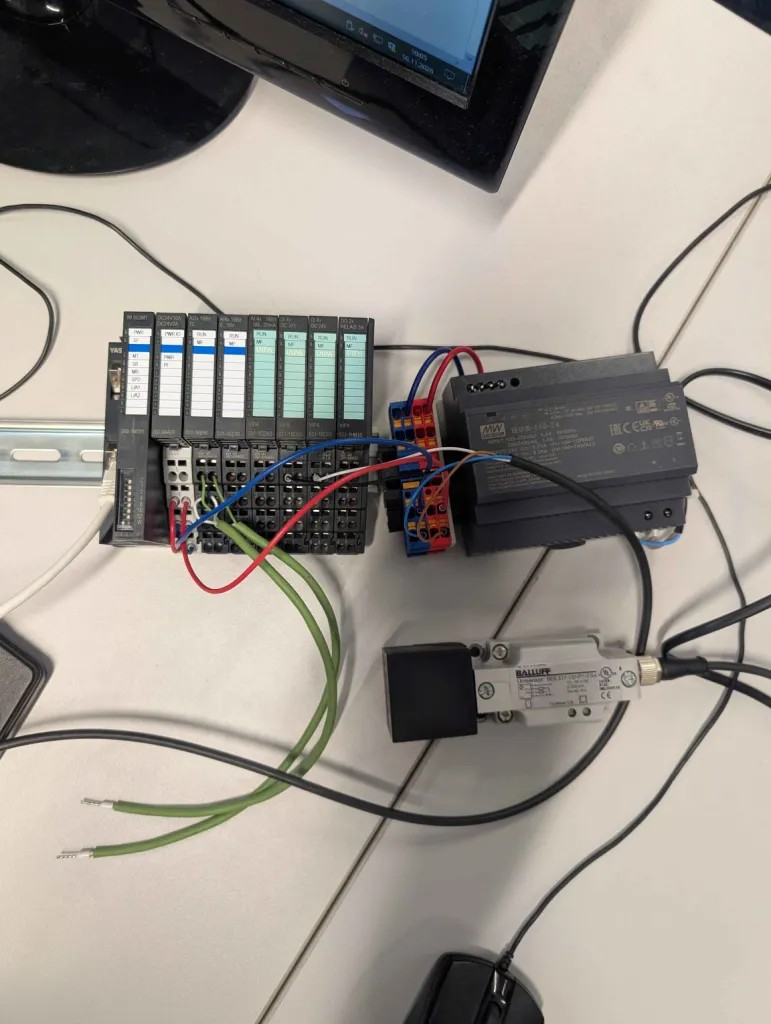
\includegraphics[width=.7\linewidth]{zapojeni_novy.jpg}
\caption{Laboratorní sestava s distribuovanými vstupy a napájením}
\label{fig:zapojeni}
\end{figure}

Dalším přístrojem byl indukční snímač Balluff BES 517-132-P7-H-S4 (obrázek~\ref{fig:senzor}). Podle štítku je určen pro napájení 10 až 55 V DC a má jmenovitou spínací vzdálenost 40 mm. Jeho stav představuje diskrétní údaj; konkrétní přiřazení vstupu a jeho zobrazení v aplikaci nejsou z podkladů jednoznačně patrné.
\begin{figure}[htbp]
\centering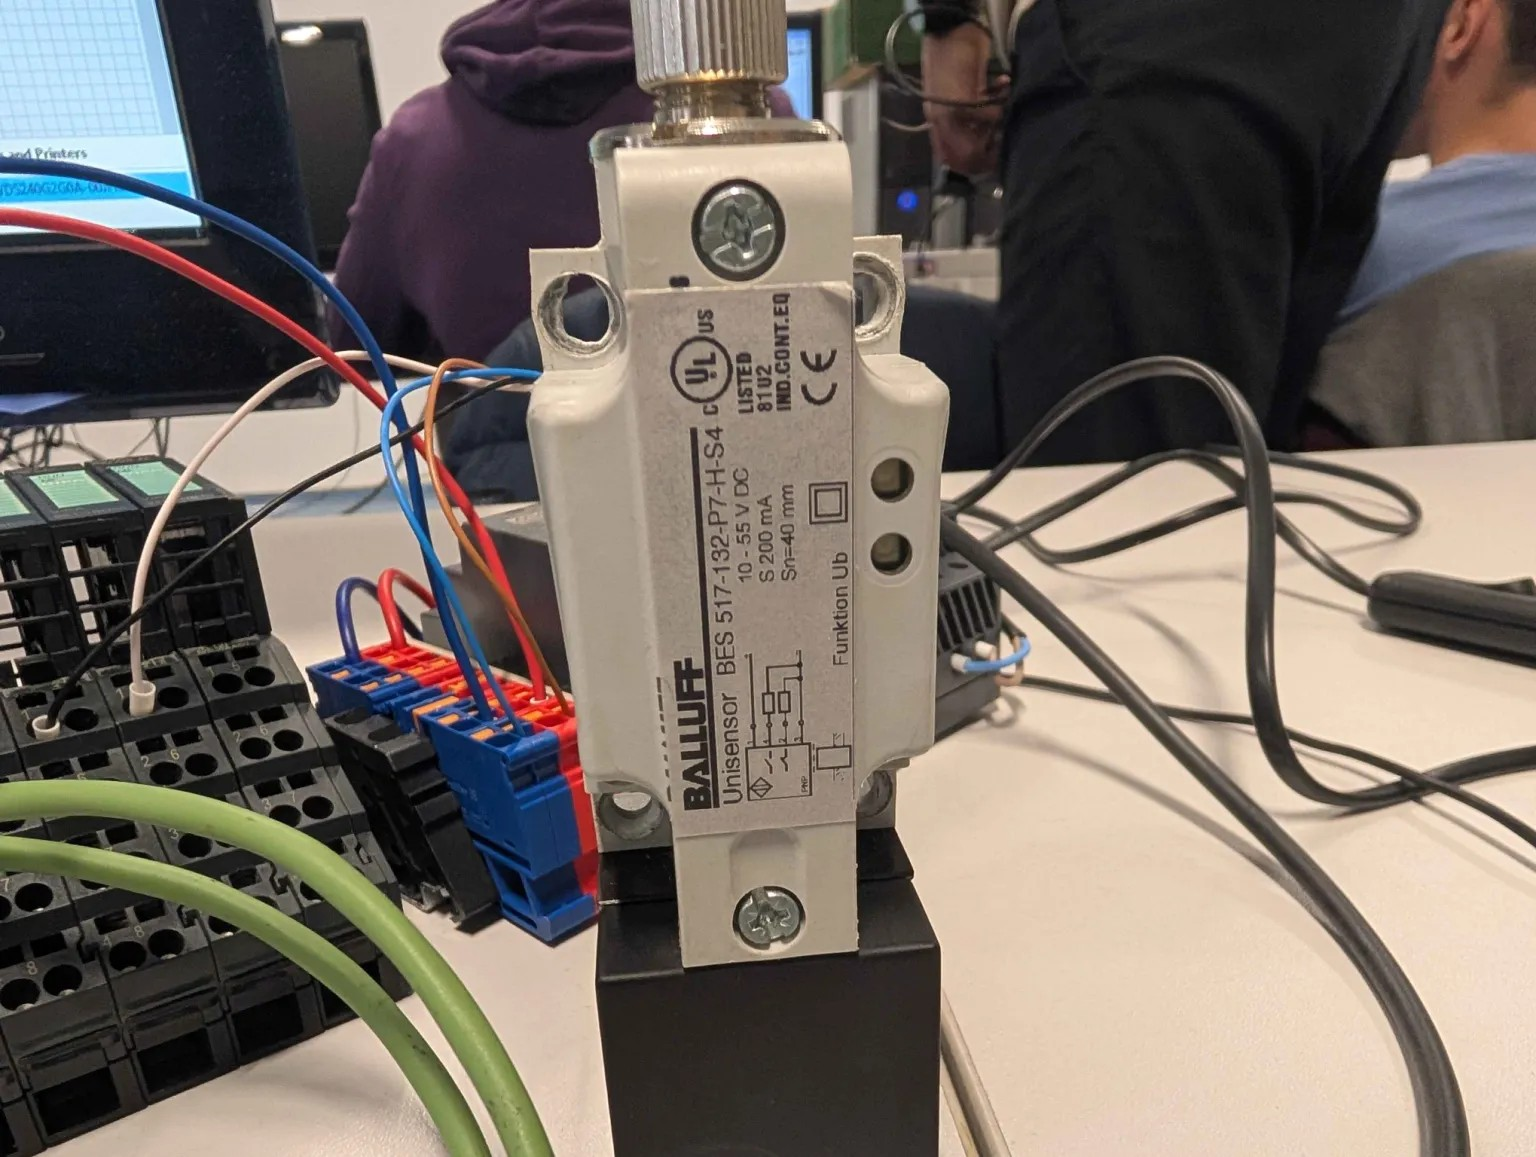
\includegraphics[width=.65\linewidth]{dalsi_merak_novy.jpg}
\caption{Indukční snímač Balluff}
\label{fig:senzor}
\end{figure}

\subsection{Komunikace a aplikace v LabVIEW}
Modbus TCP/IP umožňuje klientovi číst data dostupná v registrech síťového zařízení. V uvedené sestavě se aplikace LabVIEW připojuje k modulu Yaskawa na adrese \texttt{192.168.0.100}, která je uvedena v blokovém diagramu. Před komunikací je třeba zajistit síťovou dostupnost této adresy a odpovídající konfiguraci vstupních modulů. Podklady obsahují také snímek DHCP serveru a webového rozhraní stanice; samy o sobě však nedokládají přesný postup přidělení adresy.

\begin{figure}[htbp]
\centering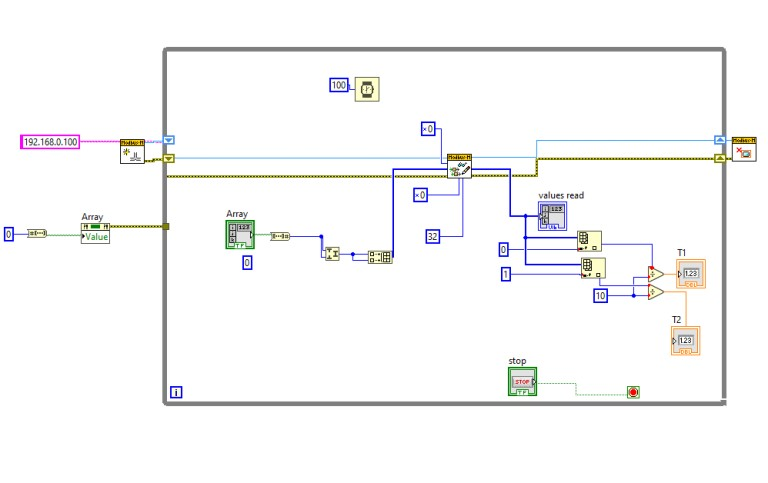
\includegraphics[width=\linewidth]{block_diagram_screen_novy.jpg}
\caption{Blokový diagram aplikace LabVIEW}
\label{fig:labview}
\end{figure}

Na obrázku~\ref{fig:labview} je připojení vytvořeno před cyklem \textit{While Loop}. V cyklu se opakovaně provádí čtení hodnot a zobrazuje se pole \textit{values read}. Z jeho prvků s indexy 0 a 1 se získávají hodnoty pro indikátory T1 a T2; obě jsou děleny deseti. Tento převod odpovídá zobrazení hodnoty uložené v desetinách jednotky. V diagramu je dále vidět konstanta 32 u čtecího bloku a čekání 100 ms mezi průchody cyklem. Tlačítko \textit{Stop} cyklus ukončí a po něm se spojení uzavře. Přesný význam všech vstupů čtecího bloku a mapu registrů nelze ze snímku bezpečně určit.

\subsection{Vyhodnocení}
Blokový diagram dokládá návrh cyklického čtení dat přes Modbus TCP/IP a zpracování dvou hodnot pro indikátory teploty. Podklady neobsahují čitelné naměřené hodnoty ani záznam ověřující změnu stavu indukčního snímače, a proto nelze doložit dosažené výsledky ani potvrdit přenos všech tří údajů. Pro úplné vyhodnocení je nutné doplnit typ termočlánků, přiřazení kanálů a registrů a naměřené hodnoty včetně stavu snímače.

\subsection{Použité přístroje}
\begin{table}[htbp]
\centering
\begin{tabular}{|p{6cm}|p{7cm}|}\hline
Přístroj & Výrobce a typ \\ \hline
Komunikační modul & Yaskawa IM053-MT01, Modbus TCP/IP \\ \hline
Indukční snímač & Balluff BES 517-132-P7-H-S4 \\ \hline
Dva termočlánky & Typ z podkladů nezjištěn \\ \hline
Vstupní moduly a napájecí zdroj & Přesné typy nejsou spolehlivě určeny \\ \hline
Počítač & LabVIEW \\ \hline
\end{tabular}
\end{table}
